\chapter{Fashion Entrepreneurs Wise Life Advice}

This short lecture is not a formal derivation, but it does unfold a definite mechanism. The speaker answers a backward-looking business question with two linked lessons: relationships create access, and customer service creates repeat business together with word of mouth. We will therefore keep the transcript order and use a small amount of notation only to make the commercial logic more explicit than ordinary prose allows.

\begin{remark}
The displayed formulas in this chapter are editorial reconstructions of the lecture's causal structure. They are not visible board equations, and they should be read as compact summaries of what the speaker says in words.
\end{remark}

\section{The Retrospective Question}

The lecture begins with a disciplined prompt: if we could go back to the beginning of the business, what are the two things we would most want to have known? That setup matters. We are not being asked for an encyclopedia of business advice, but for a ranked correction to an earlier self.

This gives the whole discussion a useful order. First comes the principle of relationships. Second comes the principle of customer service. The shortness of the interview does not make the structure loose; on the contrary, the answer is tightly staged and each later claim explains why the earlier one works.

\section{Relationships Before Technique}

The first claim arrives without ornament: relationships are the most important thing in the world. The speaker immediately compresses this into the familiar slogan that it is not what we know, but who we know. In these notes we can make that compression explicit by introducing
\[
R = \text{relationship capital},
\qquad
O = \text{downstream opportunity}.
\]
Then the speaker's first lesson may be written in the compact form
\begin{equation}
R \to O.
\end{equation}

The point is not that technical knowledge is useless. The point is that, in the commercial setting under discussion, access often arrives through persons before it arrives through systems. The lecture is therefore not making an epistemic claim about truth; it is making a practical claim about motion in the market.

A second way to summarize the same hierarchy is
\begin{equation}
O \propto R.
\end{equation}
We should read this proportion carefully. It is not a measured law. It says only that, all else equal, more trusted relationships tend to generate more openings, introductions, invitations, and chances to be seen.

\section{From Service to Opportunity}

The speaker does not leave the slogan at the level of slogan. He gives an anecdotal test case: he says that he has judged three fashion shows in the past year because of a relation that came from giving great customer service to someone else. The transcript is slightly garbled at that point, but the intended mechanism is clear enough to reconstruct cautiously.

We introduce one more symbol,
\[
S = \text{service quality},
\qquad
T = \text{remembered trust}.
\]
Then the anecdote suggests the chain
\begin{align}
S &\to T,\\
T &\to R,\\
R &\to O.
\end{align}
Composing the arrows, we obtain the speaker's implied mechanism:
\begin{equation}
S \to T \to R \to O.
\end{equation}

This is the first important clarification of the chapter. A sale is not the end of the interaction. Good service may leave behind trust, trust may stabilize into relationship, and relationship may return later in a different form from the original transaction.

\subsection{Question \& Answer}

\paragraph{Question.} How can a single act of customer service to one person later reappear as an opportunity in a quite different setting, such as a judging invitation?

\paragraph{Answer.} Because the act is not commercially exhausted at the cash register. It leaves a residue. The lecture's language is informal, but the mechanism is sharp: remembered trust travels, and when it travels through a person it becomes relationship capital.

We can write the logic as a short derivation.

\begin{enumerate}
\item An interaction of high service quality creates a positive memory.
\item A positive memory, if it persists, becomes trust rather than mere recollection.
\item Trust attached to a person becomes relationship capital.
\item Relationship capital can later be converted into access, referrals, and invitations.
\end{enumerate}

Thus the original service event has delayed commercial consequences. In the speaker's anecdote, the observed outcome is concrete rather than vague: three fashion-show judging opportunities in one year. The notes should preserve that count because it is the interview's one hard quantitative marker.

\section{Secondly: Customer Service Makes People Come Back}

The lecture then announces its hinge explicitly: ``Secondly.'' This is not a side remark. It is the second thing the speaker wishes he had known at the beginning. Here the claim is direct: customer service makes people come back, and word of mouth is the best advertising.

We introduce
\[
B = \text{return business},
\qquad
W = \text{word-of-mouth effect}.
\]
Then the second lesson may be written as
\begin{equation}
S \to B \to W.
\end{equation}

This is a stronger claim than mere politeness. Service is not only about keeping the immediate encounter pleasant; it is a generator of future traffic and future speech. In other words, the speaker is describing an aftereffect. If the first lesson told us that relationships generate access, the second tells us how such relationships are often made in the first place.

\paragraph{A worked schematic update.} To keep the lecture's logic visible across repeated interactions, let \(A_n\) be a crude indicator of authenticity at the \(n\)-th encounter, with
\[
A_n =
\begin{cases}
0, & \text{scripted courtesy},\\
1, & \text{personal service}.
\end{cases}
\]
A minimal bookkeeping model is then
\begin{align}
B_{n+1} &= B_n + \phi(A_n),\\
W_{n+1} &= W_n + \psi(B_{n+1}),
\end{align}
where \(\phi(1) > \phi(0)\) and \(\psi\) is increasing. This is not a statistical model of a store. It is only a clean way of saying what the speaker says in prose: personal treatment builds more return business than mechanical treatment, and return business feeds word of mouth.

\section{Scripted Courtesy Versus Personal Service}

Now the lecture sharpens the mechanism by contrast. Think about walking into a large store, the speaker says: we hear the routine greeting, but it has been said so many times that it no longer feels as though it comes from the heart. This is not a criticism of greeting as such. It is a distinction between a formula and a relation.

The useful variable here is authenticity:
\[
A = \text{personal quality of the interaction}.
\]
Then the closing business rule of the lecture may be summarized by
\begin{equation}
A \uparrow \;\Rightarrow\; W \uparrow.
\end{equation}
Again, this is not a measured elasticity. It is the speaker's practical judgment that memorable, sincere treatment is more likely to be repeated in speech, and therefore more likely to circulate through the market.

\begin{figure}[h]
\centering
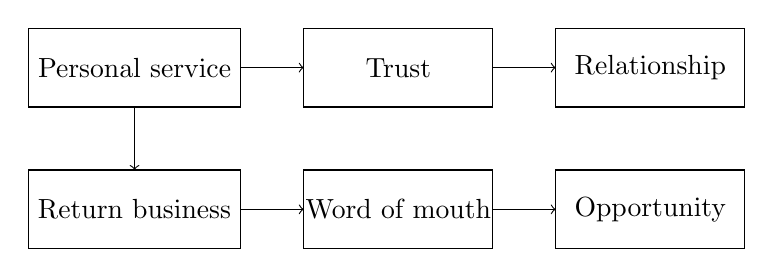
\begin{tikzpicture}[x=1cm,y=1cm]
\draw (0,0) rectangle (2.7,1) node[pos=.5]{Personal service};
\draw[->] (2.7,0.5) -- (3.5,0.5);
\draw (3.5,0) rectangle (5.9,1) node[pos=.5]{Trust};
\draw[->] (5.9,0.5) -- (6.7,0.5);
\draw (6.7,0) rectangle (9.1,1) node[pos=.5]{Relationship};
\draw[->] (1.35,0) -- (1.35,-0.8);
\draw (0,-1.8) rectangle (2.7,-0.8) node[pos=.5]{Return business};
\draw[->] (2.7,-1.3) -- (3.5,-1.3);
\draw (3.5,-1.8) rectangle (5.9,-0.8) node[pos=.5]{Word of mouth};
\draw[->] (5.9,-1.3) -- (6.7,-1.3);
\draw (6.7,-1.8) rectangle (9.1,-0.8) node[pos=.5]{Opportunity};
\end{tikzpicture}
\end{figure}

The diagram is a compact reconstruction of the lecture's two claims taken together. The top row tells us why service can become relationship. The bottom row tells us why service can become repeated trade and market speech. The final box, opportunity, closes the loop back to the speaker's anecdote about fashion-show judging.

\section{Make It Personal}

The lecture ends with a simple imperative: make it personal. We should not read this as a decorative moral flourish. It is the operational synthesis of the whole interview.

If service is generic, it may complete the transaction while leaving very little behind. If it is personal, it leaves memory; memory can become trust; trust can become relationship; and relationship can later reappear as access. The speaker's two lessons are therefore not really separate laws. They are two cuts through the same commercial process.

First, relationships matter because opportunity often comes through people. Second, customer service matters because it is one of the most reliable ways of creating the remembered trust from which such relationships grow. The lecture is short, but its logic is cumulative.

\section{Summary}

We can summarize the chapter in three linked lines. The first is that relationships generate opportunity:
\[
R \to O.
\]
The second is that customer service generates return business and word of mouth:
\[
S \to B \to W.
\]
The third is that the deeper chain runs through remembered trust:
\[
S \to T \to R \to O.
\]

In that form the interview becomes more than a set of aphorisms. It becomes a small theory of commercial causation. The practical conclusion is exactly the lecture's own conclusion: if we want the market to remember us, we must make the interaction personal.